\documentclass{article}


% if you need to pass options to natbib, use, e.g.:
\PassOptionsToPackage{numbers, compress}{natbib}
% before loading neurips_2023


% ready for submission
% \usepackage{neurips_2023}



% to compile a preprint version, e.g., for submission to arXiv, add add the
% [preprint] option:
\usepackage[preprint]{neurips_2023}


% to compile a camera-ready version, add the [final] option, e.g.:
% \usepackage[final]{neurips_2023}


% to avoid loading the natbib package, add option nonatbib:
% \usepackage[nonatbib]{neurips_2023}


% \usepackage[utf8]{inputenc} % allow utf-8 input
% \usepackage[T1]{fontenc}    % use 8-bit T1 fonts
% \usepackage{hyperref}       % hyperlinks
% \usepackage{url}            % simple URL typesetting
% \usepackage{booktabs}       % professional-quality tables
% \usepackage{amsfonts}       % blackboard math symbols
% \usepackage{nicefrac}       % compact symbols for 1/2, etc.
% \usepackage{microtype}      % microtypography
% \usepackage{xcolor}         % colors

\usepackage[utf8]{inputenc} % allow utf-8 input
\usepackage[T1]{fontenc}    % use 8-bit T1 fonts
\usepackage{hyperref}       % hyperlinks
\usepackage{url}            % simple URL typesetting
\usepackage{booktabs}       % professional-quality tables
\usepackage{amsfonts}       % blackboard math symbols
\usepackage{nicefrac}       % compact symbols for 1/2, etc.
\usepackage{microtype}      % microtypography
\usepackage{tabularx}
\usepackage{microtype}
\usepackage{graphicx}
\usepackage{subfigure}
\usepackage{booktabs} % for professional tables
\usepackage{amsmath} % For advanced math typesetting
\usepackage{amssymb} % For additional mathematical symbols
\usepackage{enumitem}
% hyperref makes hyperlinks in the resulting PDF.
% If your build breaks (sometimes temporarily if a hyperlink spans a page)
% please comment out the following usepackage line and replace
% \usepackage{icml2021} with \usepackage[nohyperref]{icml2021} above.
\usepackage{hyperref}
\usepackage[export]{adjustbox}


\title{SortFormer: Permutation Encoding for Transformer}


% The \author macro works with any number of authors. There are two commands
% used to separate the names and addresses of multiple authors: \And and \AND.
%
% Using \And between authors leaves it to LaTeX to determine where to break the
% lines. Using \AND forces a line break at that point. So, if LaTeX puts 3 of 4
% authors names on the first line, and the last on the second line, try using
% \AND instead of \And before the third author name.


\newcommand{\poemi}{\emph{Permutation Order-Equivariance Mapping-Invariance}}
\newcommand{\perminv}{\emph{Permutation Invariance}}
\newcommand{\permeq}{\emph{Permutation Equivariance}}

\newcommand\sdots{\makebox[1em][c]{.\hfil.\hfil.}}

\author{%
  Taejin Park \thanks{Use footnote for providing further information
    about author (webpage, alternative address)---\emph{not} for acknowledging
    funding agencies.} \\
NVIDIA, Santa Clara, CA, USA
  \texttt{taejinp@nvidia.com} \\
  % examples of more authors
  % \And
  % Coauthor \\
  % Affiliation \\
  % Address \\
  % \texttt{email} \\
  % \AND
  % Coauthor \\
  % Affiliation \\
  % Address \\
  % \texttt{email} \\
  % \And
  % Coauthor \\
  % Affiliation \\
  % Address \\
  % \texttt{email} \\
  % \And
  % Coauthor \\
  % Affiliation \\
  % Address \\
  % \texttt{email} \\
}


\begin{document}


\maketitle


\begin{abstract}
  We propose \textit{SortFormer} architecture, which is a Transformer variant that encodes permutation information into hidden states. We address the challenge of permutation invariance 
  in processing sequential data using Transformer architectures. Despite their effectiveness in learning and generalizing across text, speech, and image data, 
  Transformers struggle with inputs where permutations should be disregarded. This limitation often results in significant overfitting where the trained model hardly handles 
  permutations on the unseen datapoints. We identify that the inherent design of the original Transformer architecture contributes to this deficiency.
  SortFormer operates by generating estimated labels at each layer, which are then sorted according to their arrival order. These sequentially ordered labels serve as
  a permutative encoding, guiding the Transformer model in recognizing the sequence order. 
  Through ablation studies, we demonstrate that SortFormer exhibits reduced overfitting and enhanced generalization capabilities on unseen data sequences.
  Furthermore, we provide insights into the practical applicability of SortFormer in real-world scenarios. 
  Our findings suggest that this innovative architecture holds significant promise for improving the robustness and versatility of 
  Transformer models in handling permutation-sensitive sequential data.
\end{abstract}


\section{Introduction}
In recent years, the large language models (LLMs) \cite{radford2019language, rao2022megatron} gained significant popularity and most of the LLMs are based on the Transformer~\cite{vaswani2017attention}
architecture that is now being used for not only language modeling
as language understanding \cite{devlin2018bert, raffel2019learning}, GPT3~\cite{brown2020gpt3}. Other tasks such as image processing field also started leveraging
Transformers such as image generation~\cite{parmar2018image} and image recognition with ViT~\cite{dosovitskiy2020image}. In speech recognition field, Conformer~\cite{gulati2020conformer}
and Whisper~\cite{radford2023robust} successfully employed Transformer archietcture to speech-to-text (STT) tasks.

\paragraph{Transformer Variants for Efficiency}
The wide adoption of Transformer architecture also led to more efficient variants of the model such as Reformer~\cite{kitaev2019reformer},
which introduces efficient memory handling in Transformers through locality-sensitive hashing; Transformer-XL~\cite{dai2019transformer},
enhancing Transformer models for long sequence tasks with segment-level recurrence and a novel positional encoding;
Performer~\cite{choromanski2020rethinking}, offering a scalable Transformer variant with a new attention mechanism for processing long sequences efficiently;
Longformer~\cite{beltagy2020longformer}, designed for longer texts with a modified attention mechanism that combines sliding window and global attention for tasks like document classification and question answering;
SegFormer~\cite{xie2021segformer}, an approach for semantic segmentation combining a hierarchical Transformer encoder with a lightweight MLP decoder; and
RoFormer\cite{su2023roformer}, which enhances Transformer models with a rotational position encoding scheme for improved performance in various natural language processing tasks.
These variants showcase significant advancements in handling long sequences,
improving memory efficiency, and extending the applicability of Transformer models in various domains, including text and image processing.


% \paragraph{Definition 1} \emph{Permutation Function $\pi$}\\
% For a set $\mathcal{S} = \{x_1, x_2, \ldots, x_N\}$ of distinct elements, a permutation function $\pi: \mathcal{S} \rightarrow \mathcal{S}$ is a bijection. 
% The permutation function $\pi$ implies the following:
% \[ \pi(x_i) = x_j, \, \text{for all } x_i, x_j \in \mathcal{S}, \, \text{where } i, j \in \{1, 2, \ldots, N\} \text{ and } i \neq j \implies \pi(x_i) \neq \pi(x_j) \]
% The total number of permutations of $\mathcal{S}$ is $N!$ is the cardinality of the set $\mathcal{S}$.

%%%%%%%%%%%%%%%%%%%%%%%%%%%%%%%%%%%%%%%%%%%%%%%%%%%%%%%%%%%%%%%%%%%%%%%%%%
% https://www.math.ucdavis.edu/~anne/WQ2007/mat67-Lm-Determinant.pdf
%%%%%%%%%%%%%%%%%%%%%%%%%%%%%%%%%%%%%%%%%%%%%%%%%%%%%%%%%%%%%%%%%%%%%%%%%%
\paragraph{Definition 1} \emph{Permutation Function $\pi$}\\
Let $n \in \mathbb{Z}_{+}$be a positive integer. Then, mathematically, we define a permutation as any invertible bijective transformation of the finite set $\{1, \ldots, n\}$ into itself.
% A permutation $\pi$ of $n$ elements is a one-to-one and onto function having the set $\{1,2, \ldots, n\}$ as both its domain and codomain.
Thus, a permutation is a function $\pi:\{1,2, \ldots, n\} \longrightarrow\{1,2, \ldots, n\}$ such that, 
for every integer $i \in\{1, \ldots, n\}$, there exists exactly one integer $j \in\{1, \ldots, n\}$ for which 
\begin{align}
\pi(j)=i.
\end{align}
% Let $\mathcal{S} = \{x_1, x_2, \ldots, x_N\}$ be a set of $N$ distinct elements. A permutation function $\pi: \mathcal{S} \rightarrow \mathcal{S}$ is defined as a bijection, meaning that each element in $\mathcal{S}$ is mapped to a unique element in $\mathcal{S}$, and every element in $\mathcal{S}$ is the image of exactly one element in $\mathcal{S}$. Formally, the permutation function $\pi$ satisfies the following condition:
% \[ \pi(x_i) = x_{\pi(i)}, \]
% where $\pi(i)$ is the index in the permuted sequence. For any two elements $x_i, x_j \in \mathcal{S}$, if $x_i \neq x_j$, then $\pi(x_i) \neq \pi(x_j)$. This ensures that distinct elements in $\mathcal{S}$ are mapped to distinct elements under $\pi$.
% The total number of permutations of $\mathcal{S}$ is $N!$ where $N$ is the cardinality of the set $\mathcal{S}$.





\paragraph{Definition 2} \emph{Order Permutation Function $\tau$}\\
Given a length $M$ tuple $\mathbf{x} = (x_1, \sdots, x_M) $, a permutation function \(\pi\) is a bijection from the set of indices $\mathcal{S}=\{1, \sdots, M\}$ to itself.
For a tuple input, the action of order permutation function \(\tau\) on the original tuple in a reordered set $\mathbf{x_{\tau}}$  as follows:
\begin{align}
 \mathbf{x}_{\tau} = \tau\big(\mathbf{x} \big) = \tau\big( x_{1}, \sdots, x_{M} \big) = (x_{\pi(1)}, \sdots, x_{\pi(M)} )
\end{align}
where each element \( x_i \) is relocated to the position \( \pi(i) \).

\paragraph{Definition 3} \emph{Mapping Permutation Function \(\sigma\)}\\
Given a set of labeled elements \( \mathcal{S} = \{x_1, x_2, \sdots, x_N\} \), a permutation function \(\pi\) is a bijection from this set onto itself, such that \(\pi(x_n) = x_m\),
where each element \( x_n \) is mapped to the position of another element \( x_m \), where $n \neq m$.
The function takes a tuple of elements that include repetition of elements,
(e.g., $(x_1, x_2, x_2,x_3, x_3,x_1,\sdots,x_1,)$),
and maps each element to a unique element in the same set.
For a tuple input $\mathbf{x}$, the action of \(\sigma\) on an element in the set results in a reordered set as follows:
\begin{align}
  \mathbf{x_{\sigma}} = \sigma(\mathbf{x}) = \sigma\big(x_1, x_2,\sdots,x_N) = (\pi(x_1), \pi(x_2), \sdots, \pi(x_N))
\end{align}
% where each element \( x_n \) is mapped to the position of another element \( x_m \), such that \(\pi(x_n) = x_m\).
This ensures that every element \( x_n \) in the original set is uniquely associated with one and only one element \( x_m \) in the reordered set, and vice versa.

\paragraph{Property 1 (\perminv)}
\label{par:permutation_invariance}
Let $\mathcal{X}$ be a set and $\mathcal{Y}$ be a codomain. A function $f: 2^{\mathcal{X}} \rightarrow \mathcal{Y}$ is said to be \textit{permutation invariant}
if, for any subset $\{x_1, \sdots, x_M\} \subseteq \mathcal{X}$ and any permutation $\pi$ of the indices $\{1, \sdots, M\}$, the following holds:
\begin{align}
  f\left(x_1, \sdots, x_M\right) = f\left(x_{\pi(1)}, \sdots, x_{\pi(M)}\right).
\end{align}
This property means that the output of $f$ is independent of the order of the elements in its input set.

\paragraph{Property 2 (\permeq)}
\label{par:permutation_equivariance}
Let $\pi$ be a permutation of $\{1, 2, \sdots, n\}$, and let $f: \mathbb{R}^n \rightarrow \mathbb{R}^m$ be a function. Then, $f$ is said to be \emph{permutation equivariant}
if for every input $\mathbf{x} = (x_1, x_2, \sdots, x_n) \in \mathbb{R}^n$, it holds that
\begin{equation}
  f(\tau(\mathbf{x})) = \tau(f(\mathbf{x})),
\end{equation}
where $\tau(\mathbf{x})$ represents the permutation of the components of $\mathbf{x}$ according to $\tau$, and $\tau(f(\mathbf{x}))$
represents the permutation of the components of $f(\mathbf{x})$ in the same manner. Thus, equivalently, the following equality holds:
\begin{equation}
  (x_{\pi(1)}, x_{\pi(2)}, \sdots, x_{\pi(n)}) = (f(x_{\pi(1)}), f(x_{\pi(2)}), \sdots, f(x_{\pi(n)})).
\end{equation}

\paragraph{Property 3 (\poemi)}
Let $X$ be a set, and let $X^n$ denote the set of all $n$-tuples where each element belongs to $X$.
Define a function $f: X^n \rightarrow X^n$,
where \( f \) maps an \( n \)-tuple in \( X^n \) to another \( n \)-tuple in the same set.
The function $f$ is said to possess \emph{Permutation Order-Equivariance Mapping-Invariance} if and only if
for any $n$-tuple $\mathbf{x} = (x_1, x_2, \sdots, x_n)$ in $X^n$
and any permutation of $\mathbf{x}$, denoted as $\mathbf{x}_{\sigma} = (\pi(x_1), \pi(x_2), \sdots, \pi(x_n))$,
created by any bijective permutation mapping function $\sigma : X \rightarrow X$,
the following equality holds:
\begin{align}
  f(\tau(\mathbf{x})) = \tau(f(\mathbf{x})) =  \tau(f(\mathbf{x}_{\sigma})) = f(\tau(\mathbf{x_{\sigma}}))
\end{align}
where $\tau(\mathbf{x})$ and $\tau(\mathbf{x_{\sigma}})$ represents the permutation of the components of $\mathbf{x}$ and $\mathbf{x_{\sigma}}$, respectively,
as in Property \ref{par:permutation_equivariance} according to $\tau$. Similarly, $\tau(f(\mathbf{x}))$ and $\tau(f(\mathbf{x_{\sigma}}))$ represent the permutation
of the components of $f(\mathbf{x})$ and  $f(\mathbf{x_{\sigma}})$, respectively, in the same manner.

\paragraph{Example 1 (\poemi)}
From a set of $n$-tuples, $X^n$ from a set $X = \{a,b,c\}$, $\mathbf{a} = (a,a,b,b,c)$. If \emph{Permutation Order-Equivariance Mapping-Invariance} holds for a function $f$,
then the following holds:
\begin{align}
  \begin{split}
    f(\mathbf{a}) & = f(a,a,c,c,b) 
                    = f(b,b,a,a,c) 
                    = f(b,b,c,c,a) 
                    = f(c,c,a,a,b) 
                    = f(c,c,b,b,a).
  \end{split}
\end{align}

\paragraph{Permutation Invariance/Equivariance for Multi-head Attention}
The multi-head attention (MHA) architecture proposed in \cite{vaswani2017attention} is a key component of the Transformer model, which can be described as follows:
\begin{align}
  \text{MHA}(\mathbf{Q}, \mathbf{K}, \mathbf{V}) = \text{Concat}(\mathbf{O}_1, \sdots, \mathbf{O}_h) \mathbf{W}^O,
\end{align}
where $\mathbf{Q}, \mathbf{K}, \mathbf{V} \in \mathbb{R}^{n \times d}$ are the query, key, and value matrices, respectively,
and $\mathbf{W}^O \in \mathbb{R}^{hd \times d}$ is a trainable parameter matrix. And each head is defined as:
\begin{align}
  \mathbf{O}_i = \text{Attention}(\mathbf{Q} \mathbf{W}_i^Q, \mathbf{K} \mathbf{W}_i^K, \mathbf{V} \mathbf{W}_i^V),
\end{align}
where $\mathbf{W}_i^Q, \mathbf{W}_i^K, \mathbf{W}_i^V \in \mathbb{R}^{d \times d/h}$ are trainable parameter matrices.

\paragraph{Problem that SortFormer solves}
We propose a model designed for the simultaneous estimation of class presences from a sequence of input tokens.
Consider a set of frame-wise \( F \)-dimensional embedding vectors
$ \{ \mathbf{x}_t \}_{t=1}^T $, where $ \mathbf{x}_t \in \mathbb{R}^D, t = 1, 2, \sdots, T $, representing the frame index.
Given the input sequence, the model is expected to generate the estimated sequence $\{ \mathbf{y}_t \}_{t=1}^T$, where $ \mathbf{y}_t \in \mathbb{R}^K, t = 1, 2, \sdots, T $.
SortFormer is tasked with estimating the class presences \( \left\{\mathbf{y}_t\right\}_{t=1}^T \). In this context, $\mathbf{y}_t =$ {\small $\left[y_{1, t}, y_{2, t}, \sdots, y_{K, t}\right]^{\top}$}
denotes the class presences of \( K \) classes at time \( t \). SortFormer operates under the assumption that $ y_{k, t} $ is conditionally independent given the embedding vectors (features).
Therefore, Sortformer is employing \textit{Sigmoid} instead of \textit{Softmax} unlike the activation function for the output layer in \cite{vaswani2017attention,radford2019language}.
This assumption is formalized as:

\begin{align}
  P\left(\mathbf{y}_1, \sdots, \mathbf{y}_T \mid \mathbf{x}_1, \sdots, \mathbf{x}_T\right) = \prod_{k=1}^K\prod_{t=1}^T  P\left(y_{k, t} \mid \mathbf{x}_1, \sdots, \mathbf{x}_T\right).
\end{align}

Under this framework, the task at hand is construed as a multi-label classification problem, which is amenable to modeling via a neural network, denoted as  $f_{\Theta}$. The model is defined as:

\begin{align}
  \left(\mathbf{p}_1, \sdots, \mathbf{p}_T\right) = f_{\Theta}\left(\mathbf{x}_1, \sdots, \mathbf{x}_T\right),
\end{align}

where \( \mathbf{p}_t = \left[p_{1, t}, \sdots, p_{K, t}\right]^{\top} \in (0,1)^S \) represents the posterior probabilities of the presences of \( S \) classes at frame index \( t \) and f represents
the Sortformer model with parameter.
Each \( y_{k, t} \) is defined as follows depending on the value of \( p_{k, t} \):
\begin{align}
  y_{k,t} =
  \begin{cases}
    1 & \text{if } p_{k,t} > 0.5    \\
    0 & \text{if } p_{k,t} \leq 0.5
  \end{cases}
\end{align}

The estimation of class presences $\left\{\hat{\mathbf{y}}_t\right\}_{t=1}^T$ is given by:

\begin{align}
  (\hat{\mathbf{y}}_1, \sdots, \hat{\mathbf{y}}_T) & = \underset{\mathbf{y}_t \in \mathbf{Y}}{\arg\max} \big\{ P\left(\mathbf{y}_1, \sdots, \mathbf{y}_T \mid \mathbf{x}_1, \sdots, \mathbf{x}_T\right) \big\},
  \label{eq:sortformer_vector}
\end{align}
The equation \ref{eq:sortformer_vector} can be rewritten in matrix form by concatenating the vectors $ \mathbf{X} = [ \mathbf{x}_1 \mathbf{x}_2 \sdots, \mathbf{x}_T ] $,
where each column of $\mathbf{Y}$ represents the class presences at time $t$, $ \mathbf{Y} = [\mathbf{y}_1 \, \mathbf{y}_2 \, \sdots \, \mathbf{y}_T]$.
In the simplest form, the model can be represented as:
\begin{align}
  \mathbf{Y} = f_{\Theta}\left(\mathbf{X}\right),
\end{align}
where \( \mathbf{X} \in \mathbb{R}^{D \times T} \) is the input sequence and \( \mathbf{Y} \in \mathbb{R}^{K \times T} \) is a binary matrix contains an output sequence.

\paragraph{Task Description}
In this problem, the core challenge lies in the output sequence $\mathbf{Y}$, where the number of frames have non-zero $\mathbf{y}_{t}$ is determined by the model's estimation
based on the input sequence $\mathbf{X}$. Here, $\mathbf{X}$ represents an unseen type of data. The model's task is to count the number of distinct classes
within the input sequence and generate corresponding class labels for each identified class.

It is crucial to make a clearn distinction between the problem that SortFormer is tackling and the well known tasks such as clustering, identification tasks.
This problem shares similarities with clustering tasks, open-set recognition tasks where the objective is to count the number of clusters and assign labels to them. However,
there are follwing key characteristics that distinguish this problem from the aforementioned tasks:

\begin{itemize}[leftmargin=*]
  \item \textbf{Infer Unseen Data Class} The task is not a typical classification task, where the model needs to classify the unseen type of class. For example,
        in open-set face indexing, the model needs to identify the face of people that have not been seen during training time.
  \item \textbf{Multi-labels} Each token into SortFormer can have multiple labels. For example, one picture can contain multiple people's faces. Most clustering systems are not designed
        to assign multiple labels to a single data point.
  \item \textbf{Non-Event Classification} The system should detect ``class absence'', which requires the model to learn the characteristics of null-class characteristics of the feature input.
        Clustering methods typically do not accommodate cases with 'void class', where no discernible patterns exist within a given frame.
  \item \textbf{Set-based Label Assignment Loss} The model should count the number of sets and label each frame accordingly to get generic identifiers. Followingly, the loss should be
        calculated based on the set-based label assignment.
        This aspect is often handled with permutation invariant loss (PIL).
  \item \textbf{Small-scale Set Count} The task is expecting $K<10$ classes, which is a small-scale set count. Most of the neural network based clustering systems are designed
        to handle large-scale set count where $K > 1000$. This also
        decreases the burden of applying sorting algorithm on the output classes.
\end{itemize}
An illustrative example is the speaker diarization problem. In speaker diarization, the input sequence is an audio signal, and the output sequence comprises
generic identifiers (e.g., speaker1, speaker2, ..., speakerN) for each frame. However, challenges arise in frames where no speaker is present, resulting in
an output $\mathbf{y}_t$ that consists entirely of zeros. Additionally, complications occur in frames with multiple speakers, where $\mathbf{y}_t$ becomes
a binary vector containing multiple ones.

This framework is not only relevant to the speaker diarization task but is also applicable to a variety of other problems, such as
anomaly detection in time series data,
open-set recognition in image processing,
open-set facial entity indexation in video streams,
unknown language detection in natural language processing,
and new genre detection in music classification.
the following table summarizes the tasks suitable for SortFormer and their corresponding representations.

\begin{table}[h]
  \centering
  \renewcommand{\arraystretch}{1.5} % Adjust the 1.5 to increase or decrease spacing
  \begin{tabularx}{\textwidth}{p{3cm}|p{3cm}|p{2.5cm}|p{3cm}}
    \toprule
    \textbf{Task}              & \textbf{Feature Representation} & \textbf{Input Data Type} & \textbf{Output Description}                                          \\
    \hline
    Speaker Diarization        & Speaker embeddings              & Audio streams            & Identifiers for each speaker; 'no label' for silent frames           \\
    \hline
    Anomaly Detection          & Signal feature embeddings       & Time series data         & Anomaly identifiers; 'no label' for normal data points               \\
    \hline
    Open-set Face Indexation   & Face embeddings                 & Video streams            & Anonymized identifiers for each face; 'no label' for non-face frames \\
    \hline
    Unknown Language Detection & Text embeddings                 & Text data                & Language identifiers; 'no label' for unrecognizable languages        \\
    \hline
    New Genre Detection        & Music feature embeddings        & Audio tracks             & Music genre identifiers; 'no label' for unconventional genres        \\
    \bottomrule
  \end{tabularx}
  \vspace{1.5px}
  \caption{Data Analysis Tasks and their Representations}
  \label{tab:tasks}
\end{table}
Set-based label assignment loss has been widely investigated in audio signal processing field for speaker diarization tasks and source separation tasks.

\paragraph{Contributions}
The proposed method has following contributions:
\begin{itemize}[leftmargin=*]
  \item \textbf{Replace Permutation Invariant Loss} We show that sorting layers and skip connections can be used to replace permutation invariant loss (PIL) for the tasks 
  that require permutation invariance treatment. SortFormer can be trained by regular cross-entropy loss without any permutation-free mechanism.
  \item \textbf{From Passive to Active Permutation Resolution} We define the methods that apply permutation invariant treatment at the loss calculation 
  layer as passive permutation resolution. We define the methods that apply permutation invariant treatment at the encoder model architecture level as active permutation resolution.
  The active permutation resolution has not only the advantage of reducing the computational complexity during training time but also the advantage of handling long-context or streaming settings.
  \item \textbf{Improved Compatibility for Multi-modal Training} We show that the proposed architecture is designed to be trained with the other embeddings or modalities to be trained with
  a single Transformer-vairant model on top of SortFormer layer. To achieve this, Transformer encoder type of architecture is the best fit for training the entire model with a single loss and label type.
\end{itemize}


\section{Prior Works}

\paragraph{Clustering}
There have been numerous studies on making Transformer perceive longer context, model compressing for memory efficiency and sparse models. However, there have been limited number of
published work regarding general-purpose transformer variants which can handle permutation

Deep clustering~\cite{hershey2016deep} approach uses a permutation invariant objective.
The permutation invariant objective is executed by employing a $K$-dimensional embedding $V=f_\theta(x) \in \mathbb{R}^{N \times K}$, parameterized by $\theta$, such that performing some
simple clustering in the embedding space will likely lead to a partition of $\{1, \sdots, N\}$ that is close to the target one. In this work, $V=f_\theta(x)$ is based on a deep
The partition-based training requires a reference label indicator $Y=\left\{y_{n, c}\right\}$, mapping each element $n$ to each of $c$ arbitrary partition classes, so that $y_{n, c}=1$
if element $n$ is in partition $c$.
\begin{align}
  C(\theta)=\left|V V^T-Y Y^T\right|_W^2
\end{align}
This objective has been used widely, this objective has not been applied to Transformer architecture.
Moreover, clustering loss is mean sequare error loss which is different from the loss function for other tasks (e.g., cross entropy) to be trained with Transformer architecture.
In this paper, we categorize permutation-invariant loss calculation as passive permutation resolution approach, since the model itself does not have any mechanism to handle permutation.
Thus, during inference time, no permutation handling is done.


\paragraph{Permutation Invariant Neural Networks}
As opposed to passive permutation resolution, there have been a few studies on making neural networks to be permutation invariant, which can be categorized as active permutation resolution.
In active permutation resolution approaches, the model itself has a mechanism to handle permutation while making it permutation invariant or equivariant and these permutation handling mechanism happens
during both training and inference time.
The most well known approach is Deep sets~\cite{zaheer2017deep}.
In \cite{zaheer2017deep} the author proposed a permutation invariant network where a function $f(X)$ operating on a set $X$ having elements from a countable universe, is valid set function,
i.e., invariant to the permutation of instances in $X$,
iff it can be decomposed in the form $\rho\left(\sum_{x \in X} \phi(x)\right)$, for suitable transformations $\phi$ and $\rho$.
The proposed methods in Deep Sets can either handle permutation-order invariant or equivariant. 
As we discssed in the previous section, the task that SortFormer is tackling is Permutation Order-Equivariance Mapping-Invariance, not permutation order invariant.
More importantly, if we exclude positional encoding, the Transformer architecture is permutation order equivariant.

This led to permutation order invariant architecture Set Transformer \cite{lee2019set}, which employed pooling by multi-head attention (PMA)
to replace the sum or mean pooling operation for $\phi(x)$ functions in Deep Sets~\cite{zaheer2017deep}.
The author in \cite{lee2019set} compared the performance of the regular pooling methods and PMA and showed that PMA outperforms the regular mean, max or sum pooling methods.
The Set Transformer is closely related to SortFormer in the sense that both models perform clustering task.
However, Set Transformer~\cite{lee2019set} is designed to make Transformer architecture permutation order invariant, while SortFormer is designed to make Permutation Order-Equivariant Mapping-Invariant.
In addition, Set Transformer requires additional hyper parameters such as inducing points $m$ and seed vector count $k$.
Another difference is that Set Transformer is not designed to handle the non-event class nor the overlap of two classes where \textit{Softmax} is used for the output layer.
Although the problem Set Transformer is tackling is not exactly the same as SortFormer, the model can be used as a baseline model for comparison with SortFormer.
% \begin{align}
%   \operatorname{SAB}(X)    & =\operatorname{MAB}(X, X)                               \\
%   \operatorname{ISAB}_m(X) & =\operatorname{MAB}(X, H) \in \mathbb{R}^{n \times d},  \\
%   \text { where } H        & =\operatorname{MAB}(I, X) \in \mathbb{R}^{m \times d} .
% \end{align}

\paragraph{Permutation Invariant Loss}

There is another set of studies that have exactly the same objective as SortFormer with different approaches.
The concept of permutation invariant loss (PIL) or permutation invariant training (PIT) was first popularized by the two studies \cite{kolbaek2017multitalker, yu2017permutation}
for the task of speech source separation tasks which inevitably require the model to handle permutation invariant loss calculation.
Followingly, \cite{fujita2019end} adopted the concept of PIL for the task of speaker diarization, and later improved in \cite{horiguchi2022encoder} by
employing a sequence-to-sequence model to generate the attractors by training the model with PIL. While PIL shows promising results in the aforementioned tasks,
it has a few limitations compared to the sorting-based mechanism.

First, PIL requires O($N!$) time complexity with a brute-force method
or at least O($N^3$) time complexity for $N$ number of classes
to calculate the loss with the linear sum assignment algorithm that finds
the best permutation mapping between the estimated labels and ground truth labels.
This becomes a huge burden when the number of classes is large.
The sorting-based loss calculation can be done in O($Nlog(N)$) time with numerous sorting algorithms and
even can be done in O($N$) time if the sorting is based on counting sort algorithm since the keys are binary numbers.

Second, we need a special type of loss function at the output layer of the model.
This becomes a limitation when we want to train a model with a few different tasks at the same time with one ground truth.
For example, we want to train a model with speech recognition, translation and speaker diarization tasks at the same time.
The sorting-based mechanism does not demand any special loss function at the output layer; it can be trained with any loss function once the
ground truth labels are sorted.

Lastly, PIL-based models have a chance to learn the correlation between the estimated labels and the input features.
This is because the model does not have any information regarding permutation until it generates the estimated labels at the output layer.
The sorting-based mechanism alleviates the problem since the model is informed by the permutation encoding at each layer.
Thus, when it comes to streaming setup or long-context settings, PIL-trained models need to match the permutation with the old and new estimated labels,
while the sorting-based mechanism can simply assign the labels in terms of arrival orders.




\begin{figure}[ht]
  \begin{minipage}[b]{0.33\textwidth}
    \centering
    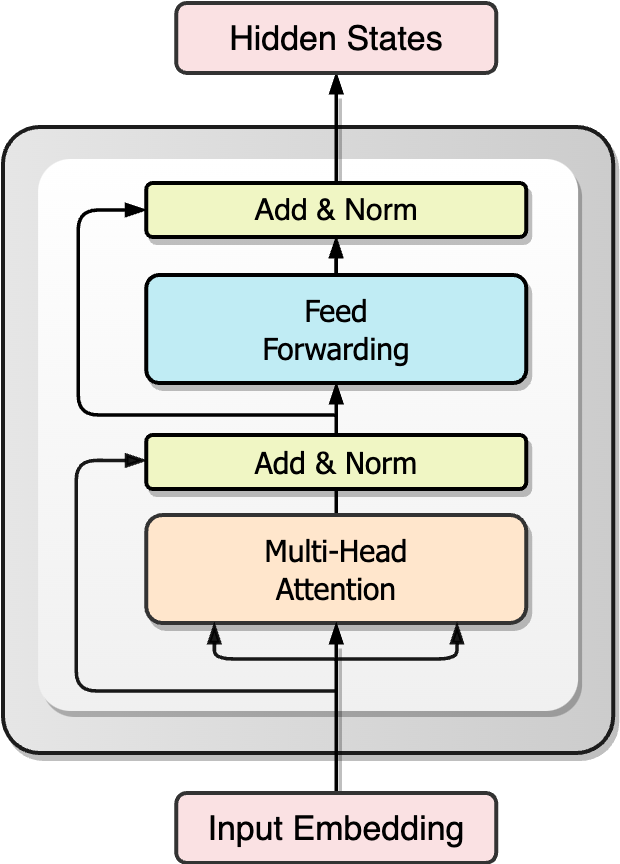
\includegraphics[width=0.73\linewidth]{pics/TransformerEncoder.drawio.png}
    \caption{Transformer Encoder}
    \label{fig:subim1}
  \end{minipage}
  \begin{minipage}[b]{0.33\textwidth}
    \centering
    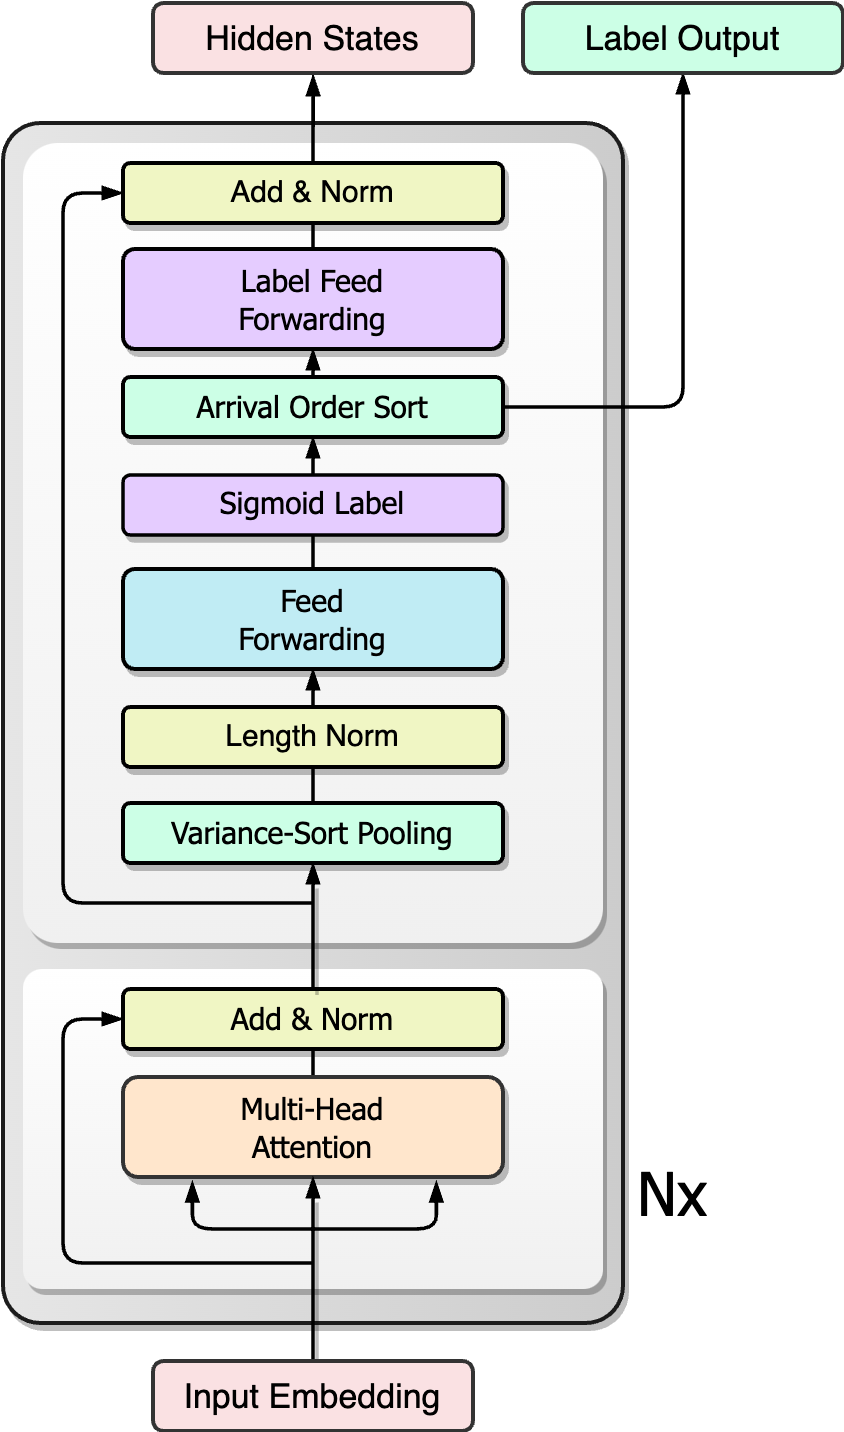
\includegraphics[width=0.9\linewidth]{pics/SortFormerEncoder.png}
    \caption{SortFormer Encoder}
    \label{fig:subim2}
  \end{minipage}
  \begin{minipage}[b]{0.33\textwidth}
    \centering
    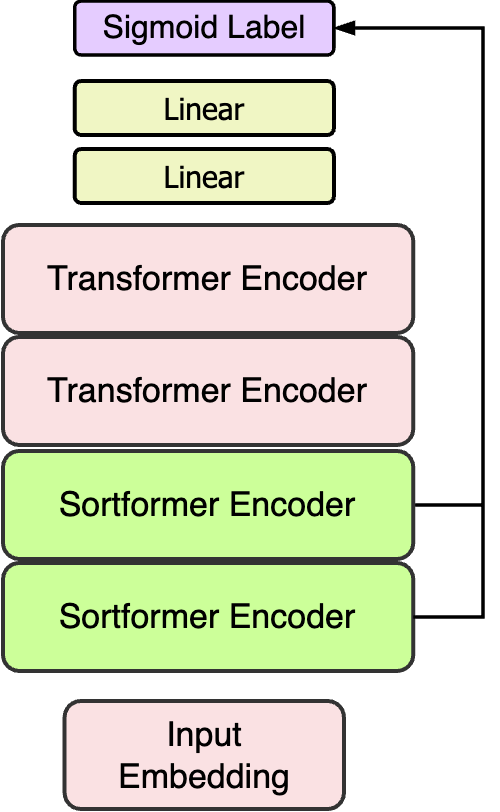
\includegraphics[width=0.5\linewidth]{pics/SortFormer_new-Page-4.drawio.png}
    \caption{SortFormer Example}
    \label{fig:subim3}
  \end{minipage}
\end{figure}

\medskip

\bibliography{sortformer}
\bibliographystyle{plainnat}

\end{document}